\section{Obstacle Avoidance}
\label{section::avoidance}

Two levels of Object avoidance were implemented and they were both taken into account when the robot decided what move to execute next. The first method used computer vision to trace straight lines; one from the robot towards the goal, and the others offset away from the first at set angles. A line tracing algorithm found in ``a Vectorial Algorithm for Tracing Straight Lines in N-Dimensional Generalized Grids''\cite{linetrace} was used. Moving outward from the robot, we determined how far in that direction the robot would be able to continue while avoiding obstacles by checking if each pixel along the line matched the table's values within tolerance.

\begin{figure}[tbp]
  \centering
  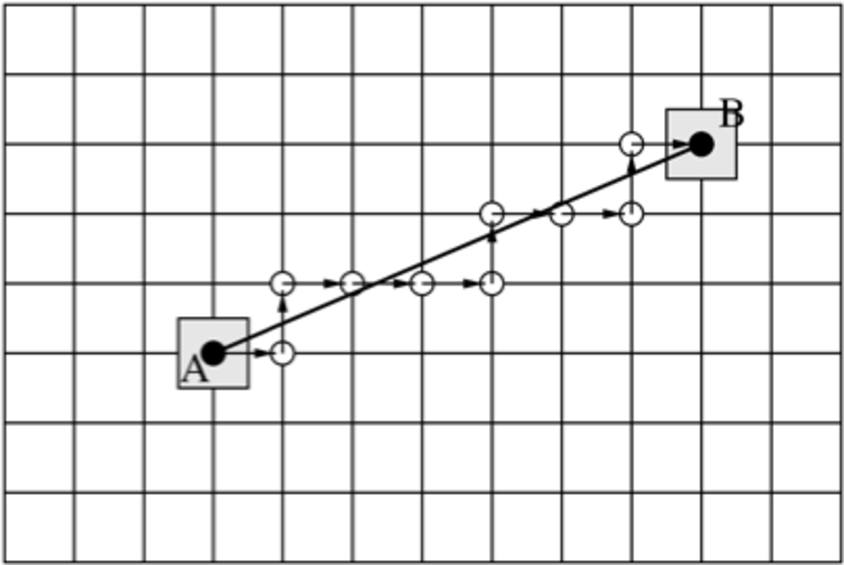
\includegraphics[width=0.5\textwidth]{media/linetrace.pdf}
  \caption{\label{line-trace} Tracing line through grid}
\end{figure}

An ultrasonic distance sensor mounted on a servomotor was used to check five different directions relative to the robot. Checking forward, and twice to each side with a set angle between each, this is similar to the vision based obstacle avoidance. This was planned to be used as a secondary method of avoiding obstacles, but turned out to be more effective, so when the values are combined it accounts for the stronger belief in the ultrasonic readings.

\begin{figure}[tbp]
  \centering
  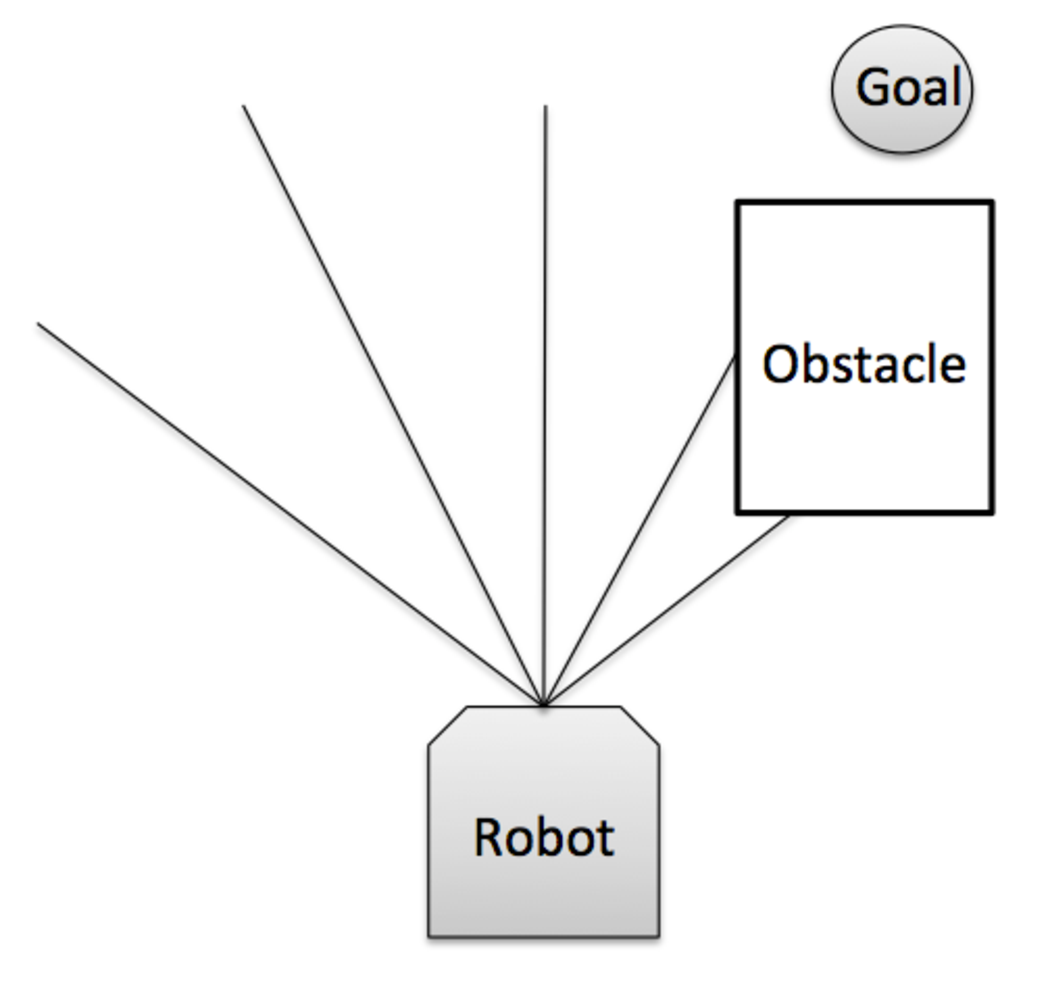
\includegraphics[width=0.5\textwidth]{media/rays.pdf}
  \caption{\label{policy-rays} Rays checked}
\end{figure}